\documentclass[10pt,a4paper]{article}

\newcommand{\cvRolle}{Senior C++/Python Backend \& Systems Engineer}
\newcommand{\cvSubheader}{High-Performance Architectures $\cdot$ Pragmatic Problem Solver $\cdot$ Domain Expert}

% ==========================================
% SETTINGS.TEX - ZENTRALE KONFIGURATION
% ==========================================
\usepackage[utf8]{inputenc}
\usepackage[T1]{fontenc}
\usepackage[american]{babel}
\usepackage[top=1.8cm, bottom=1.8cm, left=1.8cm, right=1.8cm]{geometry}
\usepackage{xcolor}
\usepackage{hyperref}
\usepackage{enumitem}
\usepackage{graphicx}
\usepackage{calc}
\usepackage{charter}
\usepackage{microtype}
\usepackage{etoolbox}

% --- DESIGN FARBEN ---
\definecolor{primary}{RGB}{15, 23, 42}      % Deep Slate / Tech Dark
\definecolor{accent}{RGB}{37, 99, 235}     % MP Blue Accent
\definecolor{textgray}{RGB}{51, 65, 85}    % Charcoal Body Text

% --- PERMANENTE ABSENDER-DATEN ---
\newcommand{\meinName}{Markus Gruber, M.Sc.}
\newcommand{\meineStrasse}{Maximilianstraße 55 Stg. B 20}
\newcommand{\meinOrt}{3100 St. Pölten}
\newcommand{\meineEmail}{Markus.Gruber4@gmx.net}
\newcommand{\meineTel}{+43 650 5871145}
\newcommand{\meinLinkedin}{https://www.linkedin.com/in/markus-gruber-70851428/}
\newcommand{\meinGithub}{https://github.com/CodeByMaxx}

% --- ROLLEN-DEFAULTS ---
\providecommand{\cvRolle}{}
\renewcommand{\cvRolle}{AI & Automation Engineer -- M&A Deal Automation}
\providecommand{\cvSubheader}{}
\renewcommand{\cvSubheader}{Python \cdot LLM APIs (OpenAI, Anthropic) \cdot Financial Data Pipelines \cdot Agent Workflows \cdot RAG}

% --- EMPFÄNGER-DATEN ---
\newcommand{\firmenName}{MP Corporate Finance}
\newcommand{\ansprechPartner}{Katharina Schwarzl-Moser (HR Manager)}
\newcommand{\firmenStrasse}{Wien, Österreich}
\newcommand{\firmenOrt}{Wien, Österreich}

% --- INTELLIGENTE ADRESS-AUSGABE (Verhindert doppelte Zeilen, wenn Straße == Ort) ---
\newcommand{\firmenAdresse}{%
    \def\tempStrasse{Wien, Österreich}%
    \def\tempOrt{Wien, Österreich}%
    \ifx\tempStrasse\tempOrt
        \tempOrt%
    \else
        Wien, Österreich \\[0.15em] Wien, Österreich%
    \fi
}

\newcommand{\stellenTitel}{AI & Automation Engineer (f/m/x)}
\newcommand{\referenzNummer}{}

\newcommand{\anrede}{Dear Ms. Schwarzl-Moser,}
\newcommand{\firmenHighlight}{MP Corporate Finance is one of Europe's leading mid-market M&A boutiques, where your AI tools will be deployed on live cross-border transactions from day one.}

% --- HEADER BEFEHL ---
\newcommand{\cvHeader}{%
\begin{center}
    {\Huge\bfseries\color{primary} \meinName}\\[0.1cm]
    {\large\bfseries \cvRolle}\\[0.05cm]
    {\color{accent}\textbf{\cvSubheader}}\\[0.1cm]
    {\small \meinOrt, Austria \quad$\cdot$\quad \meineTel \quad$\cdot$\quad \href{mailto:\meineEmail}{\meineEmail} \quad$\cdot$\quad \href{\meinLinkedin}{LinkedIn} \quad$\cdot$\quad \href{\meinGithub}{GitHub}}
\end{center}
\vspace{0.1cm}
}

% --- BEFEHLE FÜR LEBENSLÄUFE & ANSCHREIBEN ---
\newcommand{\cvsection}[1]{%
    \vspace{0.25cm}%
    {\Large\bfseries\color{primary} #1}\par%
    \vspace{-0.1cm}{\color{primary}\rule{\textwidth}{0.8pt}}\par%
    \vspace{0.15cm}%
}

\newcommand{\daterange}[2]{\hfill{\small #1 -- #2}}

% --- ENGINEERING APPROACH & MINDSET DEFINITION ---
\newcommand{\engineeringApproach}{%
    \cvsection{Engineering Approach \& Mindset}%
    \begin{itemize}[leftmargin=*, itemsep=2pt]%
        \item \textbf{Systematic Problem Solving:} First-principles analytical approach to systematic debugging and stability optimization.%
        \item \textbf{Quality & Efficiency Focus:} Pragmatic engineering mindset balancing rapid deployment with long-term maintainability and high performance.%
        \item \textbf{Cross-Functional Integration:} Acts as the technical glue bridging development, QA, and architecture.%
    \end{itemize}%
}

% --- HYPERREF SETUP ---
\hypersetup{
    colorlinks=true,
    linkcolor=primary,
    urlcolor=primary,
    pdfauthor={\meinName},
    pdftitle={Application Documents - \meinName}
}


\pagestyle{empty}

\begin{document}

\setlength{\parindent}{0pt}
\setlist[itemize]{leftmargin=1.5em, itemsep=0.15em, topsep=0.15em}

\cvHeader

\cvsection{Professional Profile}

% --- BILD LINKS, TEXT RECHTS UNTER DER ÜBERSCHRIFT ---
\begin{minipage}[t]{0.22\textwidth}
    \vspace{0pt}
    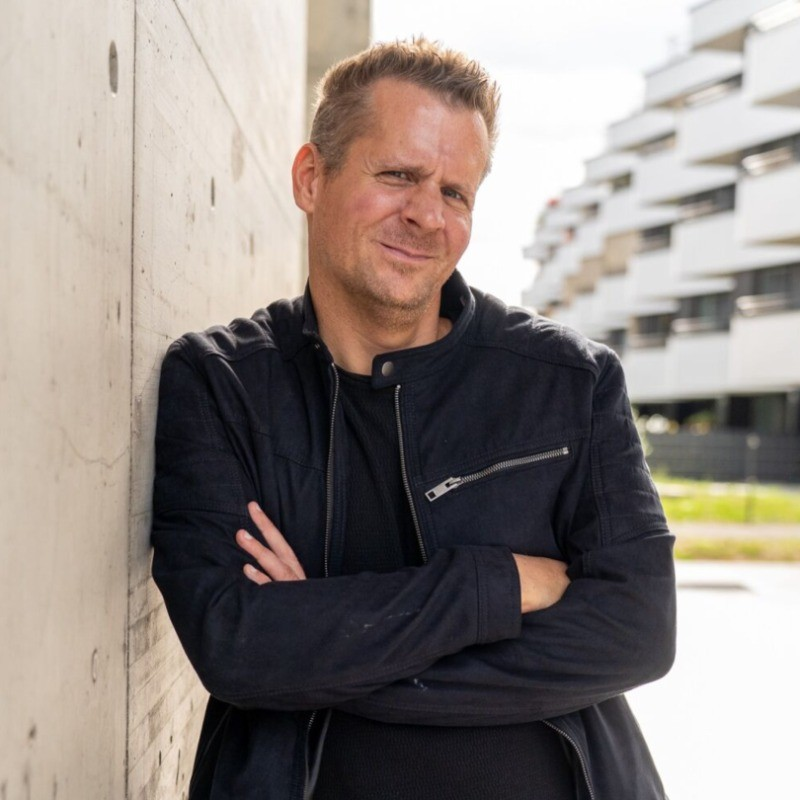
\includegraphics[width=\linewidth, keepaspectratio]{profil.jpeg}
\end{minipage}
\hfill
\begin{minipage}[t]{0.75\textwidth}
    \vspace{0pt}
    Pragmatischer Senior C++/Python Backend- \& Systems-Engineer mit über 9 Jahren Erfahrung in der Entwicklung von Echtzeit-Pipelines, Cloud-Microservices und Hochperformanten Systemen. M.Sc. in Scientific Computing mit fundiertem mathematischen Hintergrund.\\\\[0.1cm]
    Zielstrebiger Problemlöser für kritische Produktionsengpässe und Speicherlecks. Agiert als effektive Schnittstelle zwischen Entwicklung, QA und Architektur unter gezieltem Einsatz moderner KI-Tools (Cursor, Copilot).
\end{minipage}

\vspace{0.3cm}

\cvsection{Engineering Profile}

\colorbox{primary!10}{%
\parbox{\dimexpr\textwidth-2\fboxsep\relax}{%
    \vspace{0.10cm}
    \centering
    {\bfseries\color{primary} TECHNISCHES FUNDAMENT \& SYSTEMARCHITEKTUR\par}
    \vspace{0.08cm}

    \begin{minipage}[t]{0.31\linewidth}
        \raggedright
        \textbf{\color{primary}Backend Architecture}\par
        Modern C++ (11/14/17/20), Python\\
        REST APIs \& Microservices\\
        Multithreading \& Concurrency
    \end{minipage}
    \hfill
    \begin{minipage}[t]{0.31\linewidth}
        \raggedright
        \textbf{\color{primary}Systems \& Profiling}\par
        Memory Optimization \& Profiling\\
        Linux Systems \& Scripting\\
        Safety-Critical Systems (C)
    \end{minipage}
    \hfill
    \begin{minipage}[t]{0.31\linewidth}
        \raggedright
        \textbf{\color{primary}Data \& Verification}\par
        PostgreSQL, DuckDB, Redis\\
        Automated Benchmarking Suites\\
        CI/CD \& Docker Pipelines
    \end{minipage}

    \vspace{0.08cm}
}%
}

\vspace{0.15cm}

{\centering
\colorbox{accent!25}{%
\parbox{\dimexpr\textwidth-25\fboxsep\relax}{%
    \vspace{0.08cm}
    \centering
    {\bfseries\color{primary}KERN-SPEZIALISIERUNG -- BACKEND \& DISTRIBUTED SYSTEMS\par}
    \vspace{0.05cm}
    \raggedright
    \begin{itemize}[leftmargin=1.5em, itemsep=0.15em, topsep=0.15em]
        \item \textbf{\color{primary}High-Performance Backend Engineering:} Entwicklung latenzarmer Microservices, REST APIs und skalierbarer C++/Python-Execution-Engines.
        \item \textbf{\color{primary}Distributed Data Pipelines \& Systems:} Optimierung von Speicherverwaltung, nebenläufiger Verarbeitung und Datenbank-Interaktionen für produktive Workloads.
        \item \textbf{\color{primary}Automated Verification \& Telemetry:} Implementierung von End-to-End Performance-Profiling, automatisierten Benchmarking-Suiten und Telemetrie-Frameworks.
    \end{itemize}
    \vspace{0.05cm}
}%
}\par}

\cvsection{Professional Experience}

\textbf{Mindbreeze GmbH -- Software / Quality Engineer (C++/Python)} \daterange{09/2022}{07/2026}\\
\textit{C++, Python, REST APIs, Linux, Docker, Azure DevOps, Telemetry \& Performance Profiling \quad|\quad Team: 6 Engineers}
\begin{itemize}
    \item Entwicklung von Python/Bash-Automatisierungsframeworks zur Verkürzung der Release-Verifizierung von 10 auf 3 Arbeitstage.
    \item Optimierung leistungskritischer Backend-Komponenten für Unternehmensarchitekturen zur verteilten Datenverarbeitung.
    \item Refactoring von Suchmaschinen-Kernmodulen und Optimierung von Index-Datenpipelines zur Steigerung der Suchleistung.
    \item Zentraler technischer Ansprechpartner in Release-Phasen zur Behebung von Systemengpässen und Performance-
Einbußen.\end{itemize}

\vspace{0.15cm}
\textbf{Untis GmbH -- Software Engineer (C++)} \daterange{02/2022}{06/2022}\\
\textit{C++, System Refactoring, Performance Profiling, Core Desktop Modules \quad|\quad Team: 10 Engineers}
\begin{itemize}
    \item Refactoring von Legacy-C++/MFC-Kernmodulen in Visual Studio zum Abbau technischer Schulden, Optimierung der Speicherallokation und Stabilisierung des Systems.
\end{itemize}

\vspace{0.15cm}
\textbf{logi.cals -- Embedded Software Engineer (C/C++)} \daterange{02/2021}{01/2022}\\
\textit{C, C++, Embedded Systems, Safety-Critical Architectures, Deterministic Execution \quad|\quad Team: 6 Engineers}
\begin{itemize}
    \item Entwicklung deterministischer C/C++-Laufzeitsysteme (Software-SPS) und automatisierter Test-Suiten für sicherheitskritische Zertifizierungen über diverse Hardware-Plattformen hinweg.
\end{itemize}

\vspace{0.15cm}
\textbf{EYYES -- Software Engineer (C++/Python)} \daterange{04/2017}{12/2020}\\
\textit{C++, Python, Real-Time Execution Pipelines, CUDA, Embedded GPU Edge \quad|\quad Team: 8 Engineers}
\begin{itemize}
    \item Entwicklung und Implementierung KI-gestützter Bildverarbeitungspipelines (Keras, ONNX) für industrielle Echtzeit-Kamerasysteme und Edge-Computing-Plattformen.
    \item Entwicklung latenzarmer C++/CUDA-Routinen zur Performanten Echtzeit-Videoverarbeitung auf Embedded-GPUs.
    \item Implementierung hardwarenaher C++-Komponenten zur Steuerung von Kamerasensoren, Schrittmotoren und SerDes-Schnittstellen.
    \item Entwicklung, Training und Optimierung mehrerer TensorFlow-basierter Klassifikatoren zur Erreichung einer Klassifikationsgenauigkeit von 99,99 \%.
\end{itemize}

\cvsection{Selected Software Projects}

\begin{itemize}[leftmargin=1.5em, itemsep=0.2em]
    \item \textbf{Magnum C++ Game of Life:} Hochperformante C++-Simulation mit Fokus auf Low-Level-Speicherlayout, Cache-Lokalität und objektorientierte Architektur (\href{https://github.com/CodeByMaxx/magnum-game-of-life}{GitHub}).\\
    \textit{Tech: Modern C++, Memory Layout, Performance Optimization, Grid Logic}
    \item \textbf{AWS Cloud Deep Learning Pipeline:} End-to-End Cloud-Pipeline zur automatisierten Datenaufnahme und High-Throughput PyTorch-Modellinferenz (\href{https://github.com/CodeByMaxx/aws-pneumonia-detection}{GitHub}).\\
    \textit{Tech: AWS, Python, PyTorch, MLOps, REST APIs}
    \item \textbf{Azure AI Document Analyzer \& RAG Infra:} Dokumentenindexierungs- und RAG-Retrieval-Backend mit hohem Durchsatz auf Azure unter Nutzung von Vektordatenbanken (\href{https://github.com/CodeByMaxx/AI-Document-Analyzer}{GitHub}).\\
    \textit{Tech: Python, RAG, Vector DBs, Azure, Microservices}
\end{itemize}

\cvsection{Technical Skills}

\textbf{Languages \& Core:} Modern C++, C, Python, SQL, Java, Bash, Low-Level Memory Management, Parallel Algorithms, Scientific Computing.\\[0.05em]
\textbf{Architecture \& Quality:} Code Reviews, Technical Governance, Clean Code, CI/CD, Microservices, REST APIs, Performance Profiling.\\[0.05em]
\textbf{Cloud, Systems \& Infra:} Amazon AWS (S3, RDS, EC2), Microsoft Azure, Linux (Ubuntu/Debian), Windows, Docker, Kubernetes/OpenShift Basics.\\[0.05em]
\textbf{Data \& ML Infrastructure:} RAG Infrastructure, LangChain, PySpark, DuckDB, PostgreSQL, SQLAlchemy, CUDA, OpenCL.

\cvsection{Education}

\textbf{M.Sc. Scientific Computing} -- Universität Wien \daterange{10/2013}{06/2017}\\
\textit{Thesis: Silent Data Corruption in FT-GMRES (\href{https://utheses.univie.ac.at/detail/40917/}{Link}, Betreuer: Prof. Dr. W. Gansterer).}

\vspace{0.1cm}
\textbf{B.Sc. Industrial Simulation} -- FH St. Pölten \daterange{09/2010}{06/2013}\\
\textit{Thesis: Simulation of Nanocomposite Materials (\href{\meinGithub/thesis/blob/master/Bakkarbeit_final.pdf}{Link}, Betreuer: Prof. Dr. T. Schrefl).}

\newcommand{\engineeringApproachde}{%
\cvsection{Technischer Ansatz & Arbeitsweise}%
\begin{itemize}[leftmargin=*, itemsep=2pt]%
\item \textbf{Strukturierte Problemlösung:} Analytischer Ansatz auf Basis grundlegender Prinzipien zur systematischen Fehlersuche und Optimierung der Systemstabilität.%
\item \textbf{Qualitäts- und Effizienzorientierung:} Pragmatische Engineering-Mentalität, die schnelle Umsetzung mit langfristiger Wartbarkeit und hoher Leistungsfähigkeit in Einklang bringt.%
\item \textbf{Funktionsübergreifende Zusammenarbeit:} Übernimmt eine verbindende technische Rolle zwischen Entwicklung, Qualitätssicherung (QA) und Architektur.%
\end{itemize}%
}

\engineeringApproachde


\cvsection{Languages \& Work Status}

\textbf{German:} Muttersprache (C2) \quad$\cdot$\quad \textbf{English:} Verhandlungssicher (C1/C2) \quad$\cdot$\quad \textbf{Work Permit:} EU-Bürger / Österreich

\end{document}
